\section{概要}
この「じゃんけんAI」では、リアルタイムの映像から手の形を推測し、各時刻ごとに手の動きを予測しています。じゃんけんの大規模な動画データを用意するのが難しく、独自の小規模なデータで学習を行うために、学習済みの骨格推定モデルを用いて映像から手の位置や形を骨格データとして抽出し、骨格データからじゃんけんの手を推測する方法を取りました。この骨格の時系列データをもとに、次の瞬間の手の形状を予測するためにリカレントニューラルネットワーク(RNN)を活用しました。RNNの時系列予測の強みを活かし、じゃんけんの手の変化に応用することで、手を出し終わる前に予測を行い、後出しではなく自然な流れでじゃんけんができるよう工夫しています。

\section{骨格推定モデル}
骨格推定とは、人間の関節や目、鼻などの特徴点(ランドマーク)の位置を推定する技術であり、深度センサーや慣性センサーなどの高度な機器を用いた高精度な3次元推定から、通常のカメラを用いた2次元画像からの推定まで、幅広い手法が存在します。代表的な骨格推定モデルには、カーネギーメロン大学の「OpenPose」やGoogleの「MediaPipe」、および「PoseNet」などがあります。今回のじゃんけんAIでは、リアルタイムに手の動きを認識する必要があるため、「MediaPipe」 を採用しました。MediaPipeは、他のライブラリと比較して高速なリアルタイム処理に優れており、手のみの骨格推定を行うことが出来ます。手の骨格推定では、手の写った画像から21個の関節位置を検出し、深度推定を用いて3次元座標に推論することができます。
\begin{figure}[h]
  \centering
  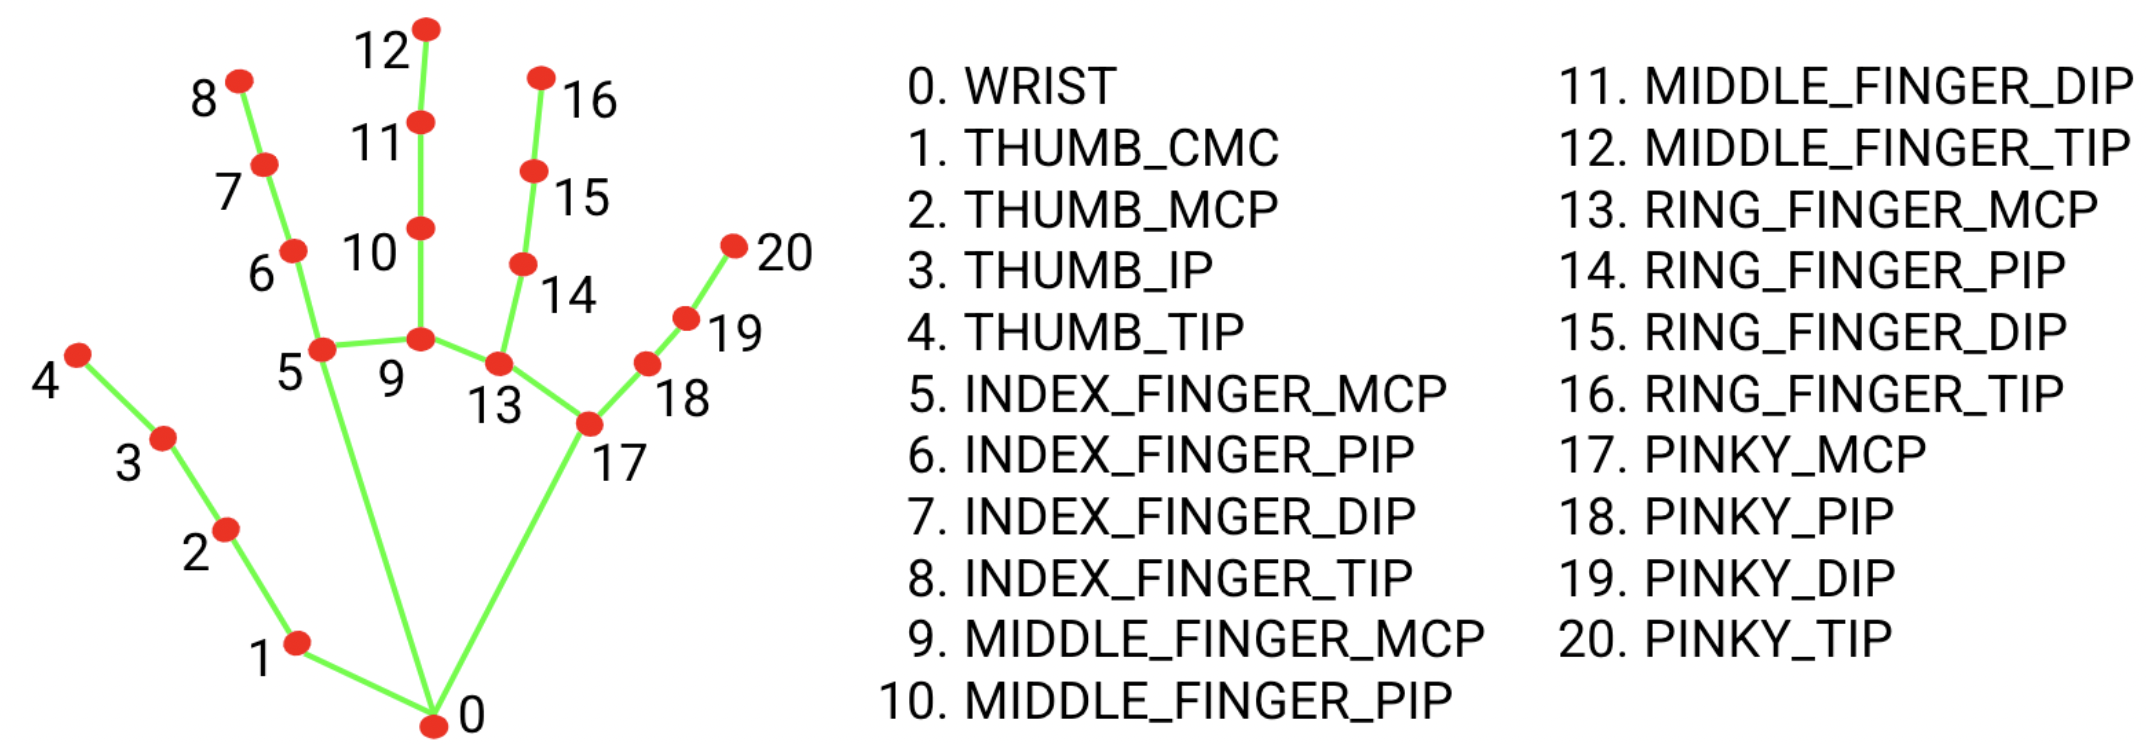
\includegraphics[width=10cm]{no-lose-janken/fig/hand-landmarks.png}
  \caption{mediapipeの検出する手の骨格}
  \label{fig:hand_landmark}
\end{figure}

\section{実験}
\subsection{データ}
学習データとして、独自に用意した246本のじゃんけん動画を使用しました。データ作成時には、多様性を確保するために、さまざまな手の握り方や角度を含めるよう意識しました。データ数が少ないため、手の平行移動を利用したデータ拡張を行ったところ、精度が大幅に向上しました。また、右手のデータのみを用いていたため、リアルタイム推論時に左手の認識がやや不安定になるという問題がありましたが、左右反転のデータ拡張を加えることで、左手も右手と同等の精度を実現しました。

\subsection{時系列予測}
骨格の時系列データの処理には、RNN・LSTM・GRUを用いて精度と推論時間の比較を行いました。時系列データを扱う強力なモデルとしてTransformerも考慮しましたが、今回は小規模なデータセットによる学習であることから使用しませんでした。

最初は、手を出す2秒前(60フレーム分)のデータで学習を行い、精度は\ref{tb:60frame}のようになりました。手を出す直前での精度はに違いは見られませんでしたが、タイミングが離れるほどRNNの精度が低下し、LSTMとGRUに関しては、1秒前まではほぼ同等の精度となりますが、2秒前になるとLSTMの方が少し精度が良くなります。しかし、学習時の2秒前の精度の高さに反し、リアルタイムで推論を行う際には、手を出す前はほとんどが「グー」となり、さらに推論が不安定になってしまいました。

手の形が変化しだすのが、手を出す約0.15秒前であることから、学習データとして手を出す瞬間の前後約0.2秒の15フレームを学習させることにしました。この15フレームでの学習では、\ref{tb:15frame}のようにRNN,LSTM,GRU全てで全時刻精度1となり、リアルタイム推論でも安定して精度よく推論できるようになりました。

\begin{table}[h]
       \hspace{0.1\textwidth}%
       \begin{subtable}{0.3\textwidth}
           \centering
           \begin{tabular}{l||c|c|r}
              & RNN & LSTM & GRU \\ \hline\hline
              2秒前 & 0.596 & 0.914 & 0.876 \\ \hline
               & 0.617 & 0.965 & 0.943 \\ \hline
               \vdots & \vdots & \vdots & \vdots \\ \hline
               & 0.684 & 0.979 & 0.980 \\ \hline
              1秒前 & 0.676 & 0.979 & 0.980 \\ \hline
               & 0.664 & 0.979 & 0.980 \\ \hline
               \vdots & \vdots & \vdots & \vdots \\ \hline
               & 0.984 & 0.985 & 0.985 \\ \hline
              ポン & 0.984 & 0.985 & 0.985 \\ \hline
           \end{tabular}
           \caption{60フレーム学習の精度比較}
           \label{tb:60frame}
       \end{subtable}%
       \hspace{0.1\textwidth}%
       \begin{subtable}{0.3\textwidth}
           \centering
           \begin{tabular}{l||c|c|r}
              & RNN & LSTM & GRU \\ \hline\hline
              -7フレーム & 1.00 & 1.00 & 1.00 \\ \hline
               & 1.00 & 1.00 & 1.00 \\ \hline
               \vdots & \vdots & \vdots & \vdots \\ \hline
               & 1.00 & 1.00 & 1.00 \\ \hline
              ポン & 1.00 & 1.00 & 1.00 \\ \hline
               & 1.00 & 1.00 & 1.00 \\ \hline
               \vdots & \vdots & \vdots & \vdots \\ \hline
               & 1.00 & 1.00 & 1.00 \\ \hline
               +7フレーム& 1.00 & 1.00 & 1.00 \\ \hline
           \end{tabular}
           \caption{15フレーム学習の精度比較}
           \label{tb:15frame}
       \end{subtable}%
   \end{table}

\subsection{推論速度}
推論速度としては全データを推論するのにかかる時間は図のようになり、全モデルでGPUよりもCPUでの推論が早く、CPUでの推論速度はRNN>GRU>LSTMとなりました。15フレームの学習では精度が変わらないので、cpuでの推論速度が一番速いRNNを採用しました。
\begin{table}[h]
           \centering
           \begin{tabular}{l||c|c|c|r}
              &RNN&LSTM&GRU\\ \hline\hline
              GPU & 241 & 202 & 243\\ \hline
              CPU & 74 & 135 & 114 \\ \hline
           \end{tabular}
           \caption{GRU}
\end{table}

\section{結論}
今回のじゃんけんAIでは、時系列予測を活用して後出しではない自然な動作を目指し、最終的に手を出し終わる前に正しい手を予測するモデルを開発することが出来ました。しかし、実際にじゃんけんをする際には、画面とのタイミングを人間側で合わせるのが難しく、モデル以外の部分に課題が残ります。今後は、人とAIのタイミングをさらに自然にする工夫を加え、よりスムーズなじゃんけんAIを目指していきたいと思います。
